\documentclass[11pt,a4paper]{scrartcl}

% ---------- pagina ----------
\usepackage[a4paper,margin=2.6cm]{geometry}
\usepackage[T1]{fontenc}
\usepackage[utf8]{inputenc}
\usepackage{amsmath,amssymb}
\usepackage{tikz}
\usetikzlibrary{arrows.meta,angles,quotes,calc,decorations.markings}
\usepackage[most]{tcolorbox}
\usepackage{xcolor}
\usepackage{enumitem}

% ---------- box "Esercizio" in stile OpenStax ----------
\newtcolorbox{esercizio}[1][]{%
  enhanced,
  breakable,
  colback=white,
  colframe=black,
  boxrule=0.6pt,
  sharp corners,
  left=2mm,right=2mm,top=1.5mm,bottom=1.5mm,
  before skip=4mm, after skip=3mm,
  #1
}

% ---------- comandi rapidi ----------
\newcommand{\N}{\ \text{N}}
\newcommand{\NC}{\ \text{N/C}}
\newcommand{\C}{\ \text{C}}
\renewcommand{\deg}{^\circ}

\newenvironment{soluzione}{\par\noindent\textbf{Soluzione ---} }{\par}
\newenvironment{riflessione}{\par\noindent\textit{\textbf{Per riflettere ---} }}{\par}

\title{\bfseries Esercizi --- Linee di forza e flusso del campo elettrico}
\author{4A --- 28/09/2026}
\date{}

\begin{document}
\maketitle
\vspace{-1.2em}

\bigskip

\subsection*{Esercizio 1 --- Le linee di $+2Q$ e $-Q$}

\begin{esercizio}
\emph{Disegnate le linee di forza di due cariche, $+2Q$ e $-Q$, con 8 linee per ogni $Q$.
Quante linee partono da $+2Q$? Quante arrivano su $-Q$? Quante vanno all'infinito?}
\end{esercizio}

\begin{soluzione}
$+2Q$ ha il doppio della carica dell'unità di riferimento, quindi genera $2\times8=16$ linee
uscenti. $-Q$, in modulo pari a un'unità, ne assorbe 8. Delle 16 linee uscenti da $+2Q$, 8
terminano su $-Q$ (bilanciando esattamente la sua carica) e le restanti 8 vanno all'infinito.

\textbf{Risposte:} 16 linee partono da $+2Q$ $\cdot$ 8 arrivano su $-Q$ $\cdot$ 8 vanno all'infinito.
\end{soluzione}

\begin{riflessione}
il criterio guida è ``il numero di linee è proporzionale alla carica, e ogni linea che nasce su
una carica positiva deve terminare su una negativa o andare all'infinito''. Nota che se avessi
fatto terminare tutte e 16 le linee su $-Q$, staresti implicitamente assegnando a $-Q$ lo stesso
modulo di carica di $+2Q$: un modo rapido per accorgersi dell'errore è controllare che il numero di
linee resti sempre coerente con il rapporto reale fra le cariche in gioco.
\end{riflessione}

\bigskip\hrule\bigskip

\subsection*{Esercizio 2 --- Una calotta semisferica in un campo uniforme}

\begin{esercizio}
\emph{Una calotta semisferica di raggio $10\ \text{cm}$ è in un campo uniforme di
$2{,}0\times10^3\NC$ parallelo al suo asse. Calcolate il flusso attraverso la calotta (normale
uscente). Che cosa cambia se la ruotate di $90\deg$?}
\end{esercizio}

\begin{center}
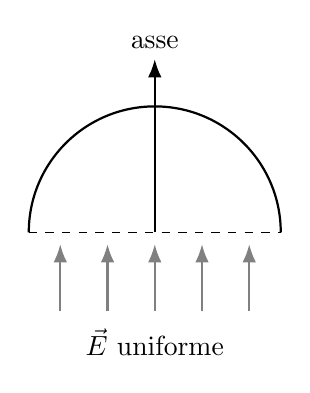
\begin{tikzpicture}[scale=1.0, >=Latex]
  \draw[thick] (-1.6,0) arc[start angle=180,end angle=0,x radius=1.6,y radius=1.6];
  \draw[dashed] (-1.6,0) -- (1.6,0);
  \draw[->,thick] (0,0) -- (0,2.2) node[above]{asse};
  \foreach \x in {-1.2,-0.6,0,0.6,1.2}{
    \draw[->,thick,gray] (\x,-1.0) -- (\x,-0.15);
  }
  \node[below] at (0,-1.1) {$\vec E$ uniforme};
\end{tikzpicture}
\end{center}

\begin{soluzione}
\textbf{Il punto chiave: non calcoliamo il flusso della calotta direttamente, ma lo ricaviamo da
una superficie chiusa.} Chiudiamo la calotta con il disco piatto che ne è il bordo (il cerchio
equatoriale di raggio $10\ \text{cm}$): calotta + disco formano insieme una superficie
\emph{chiusa} (una mezza-palla sigillata). Dentro questa superficie chiusa non c'è nessuna carica,
quindi il suo flusso totale è nullo:
\begin{equation}
  \Phi_{\text{tot}} = \Phi_{\text{calotta}} + \Phi_{\text{disco}} = 0
  \quad\Longrightarrow\quad
  \Phi_{\text{calotta}} = -\Phi_{\text{disco}}
\end{equation}
Il flusso attraverso il disco, perpendicolare al campo (l'asse della calotta è parallelo al
campo), si calcola subito:
\begin{equation}
  \Phi_{\text{disco}} = E\cdot\pi r^2 = (2{,}0\times10^3)(\pi)(0{,}10)^2 \approx 63\ \text{N}\,\text{m}^2/\text{C}
\end{equation}
(con normale uscente dalla mezza-palla, cioè verso il basso, opposta al campo: $\Phi_{\text{disco}}<0$
se orientata così). Quindi $\Phi_{\text{calotta}} \approx +63\ \text{N}\,\text{m}^2/\text{C}$ con
normale uscente verso l'alto.

Perché torna anche intuitivamente: il campo è uniforme e verticale, e non ci sono cariche dentro la
mezza-palla che creino o assorbano linee di campo. Ogni linea che entra dal disco in basso deve
quindi uscire da qualche parte sulla calotta sopra di essa --- nessuna linea può nascere o sparire
nel vuoto.

\textbf{Ruotando di $90\deg$:} l'asse della calotta diventa perpendicolare al campo, quindi il
piano del disco-bordo diventa \emph{parallelo} al campo (il campo giace nel piano del bordo). La
normale al disco è allora perpendicolare al campo, $\Phi_{\text{disco}}=0$, e per lo stesso
argomento anche $\Phi_{\text{calotta}} = \mathbf{0}$.
\end{soluzione}

\begin{riflessione}
il passaggio cruciale --- sostituire una superficie scomoda (curva) con una comoda (piatta) che
condivide lo stesso bordo, usando una superficie chiusa senza carica interna come garanzia che le
due diano lo stesso flusso in modulo --- è esattamente il trucco che regge la dimostrazione del
teorema di Gauss per la sfera: si sceglie sempre la superficie più comoda da calcolare, mai quella
``vera''. Attenzione a due errori tipici: calcolare $E\cdot A_{\text{calotta}}$ usando l'area reale
della semisfera ($2\pi r^2$) invece dell'area del disco proiettato; oppure dimenticare che
l'argomento ``flusso totale nullo'' vale solo per la coppia (calotta + disco) presa insieme, non
per la calotta isolata.
\end{riflessione}

\bigskip\hrule\bigskip

\subsection*{Esercizio 3 --- Sfera più grande}

\begin{esercizio}
\emph{Una carica $Q$ è al centro di una sfera. Se raddoppio il raggio della sfera, cosa succede al
flusso? E al campo sulla superficie?}
\end{esercizio}

\begin{center}
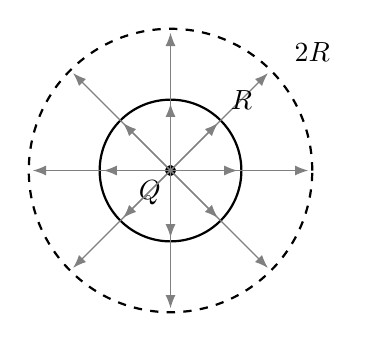
\begin{tikzpicture}[scale=1.0, >=Latex]
  \draw[thick] (0,0) circle (0.9);
  \draw[thick,dashed] (0,0) circle (1.8);
  \fill (0,0) circle (2pt) node[below left]{$Q$};
  \foreach \a in {0,45,...,315}{
    \draw[->,gray] (0,0) -- (\a:0.85);
    \draw[->,gray] (0,0) -- (\a:1.75);
  }
  \node at (0.9,0.9) {$R$};
  \node at (1.8,1.5) {$2R$};
\end{tikzpicture}
\end{center}

\begin{soluzione}
il flusso attraverso la sfera dipende solo dalla carica racchiusa, non dal raggio: raddoppiando $R$
il flusso resta \textbf{invariato}. Il campo sulla superficie, invece, scala come $1/R^2$ (legge di
Coulomb): raddoppiando $R$ il campo diventa $1/4$ del valore precedente.
\end{soluzione}

\begin{riflessione}
è l'esercizio-chiave che separa i due concetti che si tende a confondere: flusso (proprietà
globale, legata solo alla carica interna) e campo (proprietà locale, punto per punto, che dipende
dalla distanza). È esattamente il fatto che rende sensato il teorema di Gauss: il prodotto $E\cdot A$
resta costante al variare di $R$ perché $E$ cala come $1/R^2$ mentre $A$ cresce come $R^2$.
\end{riflessione}

\bigskip\hrule\bigskip

\subsection*{Esercizio 4 --- Carica fuori}

\begin{esercizio}
\emph{Una carica positiva sta vicinissima a una sfera, ma fuori. Il flusso netto attraverso
la sfera è positivo, negativo o nullo?}
\end{esercizio}

\begin{soluzione}
\textbf{Nullo.} Il teorema di Gauss conta solo le cariche racchiuse dalla superficie: una carica
esterna, per quanto vicina, contribuisce con flusso netto zero attraverso qualunque superficie
chiusa. Localmente il campo della carica esterna non è nullo sulla sfera (attraversa la superficie
con linee che entrano da un lato), ma ogni linea che entra da una parte della sfera esce dall'altra:
il computo netto si annulla.
\end{soluzione}

\begin{riflessione}
``vicinissima'' è la parola-trappola: la vicinanza rende grande il campo locale in quella zona della
sfera, ma non introduce carica racchiusa, quindi non altera il flusso netto. È il contro-esempio
naturale all'intuizione ``più vicino = più flusso''. Tienilo in mente per quando generalizzeremo
questo ragionamento a superfici non sferiche, il 28/10, con la legge di Gauss per il campo
magnetico $\vec B$.
\end{riflessione}

\bigskip\hrule\bigskip

\subsection*{Esercizio 6 --- Punto medio}

\begin{esercizio}
\emph{Due cariche uguali e positive sono a distanza $d$. Nel loro punto medio $E=0$. Passa
una linea di forza per quel punto?}
\end{esercizio}

\begin{soluzione}
\textbf{No.} Una linea di forza, per definizione, è tracciata seguendo in ogni punto la direzione
del campo. In un punto dove $E=0$ il campo non ha una direzione definita, quindi nessuna linea di
forza può passare esattamente per quel punto: è un punto di equilibrio (le linee provenienti dalle
due cariche si avvicinano e si ``annullano'' a vicenda in quella zona, senza mai toccare il punto
stesso).
\end{soluzione}

\begin{riflessione}
il punto di campo nullo fra due cariche è un'idea ricorrente in elettrostatica: qui la incontri
sulla rappresentazione grafica delle linee di forza, ma è la stessa logica di ogni punto di
equilibrio calcolato numericamente fra due cariche (uguali o disuguali). Un errore diffuso è
rispondere ``sì, ci passano tutte le linee che si scontrano lì'', confondendo il punto di arrivo
apparente del disegno con un punto realmente attraversato da una linea: nel disegno le linee si
avvicinano sempre di più al punto centrale senza mai raggiungerlo.
\end{riflessione}

\end{document}
